\documentclass[a4paper]{article}

\usepackage[T1]{fontenc}
\usepackage[utf8]{inputenc}
\usepackage{mlmodern}

%\usepackage{ngerman}	% Sprachanpassung Deutsch

\usepackage{graphicx}
\usepackage{geometry}
\geometry{a4paper, top=15mm}

\usepackage{subcaption}
\usepackage[shortlabels]{enumitem}
\usepackage{amssymb}
\usepackage{amsthm}
\usepackage{amsmath}
\usepackage{mathtools}
\usepackage{braket}
\usepackage{bbm}
\usepackage{graphicx}
\usepackage{float}
\usepackage{yhmath}
\usepackage{tikz}
\usepackage{scratch}
\usetikzlibrary{patterns,decorations.pathmorphing,positioning}
\usetikzlibrary{calc,decorations.markings}

\usepackage[backend=biber, sorting=none]{biblatex}
\addbibresource{cite.bib}

\usepackage[framemethod=TikZ]{mdframed}

\tikzstyle{titlered} =
    [draw=black, thick, fill=white,%
        text=black, rectangle,
        right, minimum height=.7cm]


\usepackage[colorlinks=true,naturalnames=true,plainpages=false,pdfpagelabels=true]{hyperref}
\usepackage[parfill]{parskip}
\usepackage{lipsum}

\usepackage{tcolorbox}
\tcbuselibrary{skins,breakable}

\pagestyle{myheadings}

\colorlet{colexam}{black}
\newcounter{definition}
\newtcolorbox[use counter=definition]{mydef}[1]{
    empty,
    title={\textbf{Definition~\thetcbcounter}~~(\textit{#1})},
    attach boxed title to top left,
    fontupper=\sl,
    boxed title style={
        empty,
        size=minimal,
        bottomrule=1pt,
        top=1pt,
        left skip=0cm,
        overlay=
            {\draw[colexam,line width=1pt]([yshift=-0.4cm]frame.north
        west)--([yshift=-0.4cm]frame.north east);}},
            coltitle=colexam,
            fonttitle=\normalfont,
            before=\par\medskip\noindent,
            parbox=false,
            boxsep=-1pt,
            left=0.75cm,
            right=3mm,
            top=4pt,
            breakable,
            pad at break*=0mm,
            vfill before first,
            overlay unbroken={
                \draw[colexam,line width=1pt]
                ([xshift=0.6cm, yshift=-0.5pt]frame.south
                west)--([xshift=0.6cm,yshift=-1pt]frame.north west)
                --([xshift=0.6cm]frame.south west)--([xshift=-13cm]frame.south east); },
            overlay first={
                \draw[colexam,line width=1pt]
                ([xshift=0.6cm, yshift=-0.5pt]frame.south
                west)--([xshift=0.6cm,yshift=-1pt]frame.north west)
                --([xshift=0.6cm]frame.south west); },
            overlay last={
                \draw[colexam,line width=1pt]
                ([xshift=0.6cm, yshift=-0.5pt]frame.south
                west)--([xshift=0.6cm,yshift=-1pt]frame.north west)
                --([xshift=0.6cm]frame.south west)--([xshift=-13cm]frame.south east); }
}
\newcounter{theorem}
\newtcolorbox[use counter=theorem]{theorem}{
    empty,
    title={Theorem ~\thetcbcounter},
    attach boxed title to top left,
    fontupper=\sl,
    boxed title style={
        empty,
        size=minimal,
        bottomrule=1pt,
        top=1pt,
        left skip=0cm,
        overlay=
            {\draw[colexam,line width=1pt]([yshift=-0.4cm]frame.north
        west)--([yshift=-0.4cm]frame.north east);}},
            coltitle=colexam,
            fonttitle=\bfseries,
            before=\par\medskip\noindent,
            parbox=false,
            boxsep=-1pt,
            left=0.75cm,
            right=3mm,
            top=4pt,
            breakable,
            pad at break*=0mm,
            vfill before first,
            overlay unbroken={
                \draw[colexam,line width=1pt]
                ([xshift=0.6cm, yshift=-0.5pt]frame.south
                west)--([xshift=0.6cm,yshift=-1pt]frame.north west)
                --([xshift=0.6cm]frame.south west)--([xshift=-13cm]frame.south east); },
            overlay first={
                \draw[colexam,line width=1pt]
                ([xshift=0.6cm, yshift=-0.5pt]frame.south
                west)--([xshift=0.6cm,yshift=-1pt]frame.north west)
                --([xshift=0.6cm]frame.south west); },
            overlay last={
                \draw[colexam,line width=1pt]
                ([xshift=0.6cm, yshift=-0.5pt]frame.south
                west)--([xshift=0.6cm,yshift=-1pt]frame.north west)
                --([xshift=0.6cm]frame.south west)--([xshift=-13cm]frame.south east); }
}
\newcounter{lemma}
\newtcolorbox[use counter=lemma]{lemma}{
    empty,
    title={Lemma~\thetcbcounter},
    attach boxed title to top left,
    fontupper=\sl,
    boxed title style={
        empty,
        size=minimal,
        bottomrule=1pt,
        top=1pt,
        left skip=0cm,
        overlay=
            {\draw[colexam,line width=1pt]([yshift=-0.4cm]frame.north
        west)--([yshift=-0.4cm]frame.north east);}},
            coltitle=colexam,
            fonttitle=\bfseries,
            before=\par\medskip\noindent,
            parbox=false,
            boxsep=-1pt,
            left=0.75cm,
            right=3mm,
            top=4pt,
            breakable,
            pad at break*=0mm,
            vfill before first,
            overlay unbroken={
                \draw[colexam,line width=1pt]
                ([xshift=0.6cm, yshift=-0.5pt]frame.south
                west)--([xshift=0.6cm,yshift=-1pt]frame.north west)
                --([xshift=0.6cm]frame.south west)--([xshift=-13cm]frame.south east); },
            overlay first={
                \draw[colexam,line width=1pt]
                ([xshift=0.6cm, yshift=-0.5pt]frame.south
                west)--([xshift=0.6cm,yshift=-1pt]frame.north west)
                --([xshift=0.6cm]frame.south west); },
            overlay last={
                \draw[colexam,line width=1pt]
                ([xshift=0.6cm, yshift=-0.5pt]frame.south
                west)--([xshift=0.6cm,yshift=-1pt]frame.north west)
                --([xshift=0.6cm]frame.south west)--([xshift=-13cm]frame.south east); }
}

\newcommand{\eps}{\varepsilon}
\usepackage[OT2,T1]{fontenc}
\DeclareSymbolFont{cyrletters}{OT2}{wncyr}{m}{n}
\DeclareMathSymbol{\Sha}{\mathalpha}{cyrletters}{"58}

\markright{Popović\hfill Seminar\hfill}


\title{University of Vienna\\
\vspace{1cm}Seminar:\\Joint RICAM Seminar\\
\vspace{0.5cm}
Summary of talk by Otmar Scherzer
}
\author{Milutin Popovic}


\usepackage{amsmath}
\numberwithin{equation}{section}

\begin{document}

\maketitle
\tableofcontents

\section{Governing Equations of Fluid Dynamics}
We first start of with a fluid with a density
\begin{align}
    \rho(\mathbf{x}, t),
\end{align}
in three dimensional Cartesian coordinates $\mathbf{x} = (x, y, z)$ at time
$t$. For water-wave applications, we should note that we take
$\rho=\text{constant}$, but we will go into this fact later. The fluid moves
in time and space with a velocity field
\begin{align}
    \mathbf{u}(\mathbf{x}, t) = (u, v, w).
\end{align}
Additionally it is also described by its pressure
\begin{align}
    P(\mathbf{x}, t),
\end{align}
generally depending on time and position. When thinking of e.g. water the
pressure increases the deeper we go, that is with decreasing or increasing $z$
direction (depending how we set up our system $z$ pointing up or down
respectively).

The general assumption in fluid dynamics is the \textbf{Continuum
Hypothesis}, which assumes continuity of $\textbf{u}, \rho$ and $P$ in
$\mathbf{x}$ and $t$. In other words, we premise that the velocity field,
density and pressure are ''nice enough`` functions of position and time, such
that we can do all the differential operations we desire in the framework of
differential analysis.
\subsection{Mass Conservation}
Our aim is to derive a model of the fluid and its dynamics, with respect to
time and position, in the most general way. This is usually done thinking
of the density of a given fluid, which is a unit mass per unit volume,
intrinsically  an integral representation to derive these equations suggests
by itself.

Let us now thing of an arbitrary fluid. Within this fluid we define a fixed
volume $V$ relative to a chosen inertial frame and bound it by a surface $S$
within the fluid, such that the fluid motion $\mathbf{u}(\mathbf{x}, t)$ may
cross the surface $S$. The fluid density is given by $\rho(\mathbf{x}, t)$,
thereby the mass of the fluid in the defined Volume $V$ is an integral
expression
\begin{align}
    m = \int_V \rho(\mathbf{x}, t) dV.
\end{align}
The figure bellow \ref{fig:volume}, expresses the above described picture.
\begin{figure}[H]
    \centering
  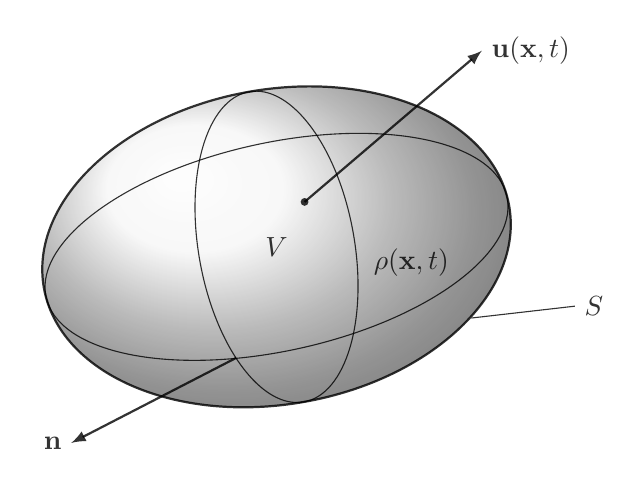
\begin{tikzpicture}[>=latex,scale=1, xscale=1, opacity=.8]
% second sphere
    \begin{scope}[rotate=10, xscale=3, yscale=2, shift={(2.3,-0.2)}]
      \coordinate (O) at (0,0);
      \shade[ball color=gray!10!] (0,0) coordinate(Hp) circle (1) ;

      \draw[thick] (O) circle (1);
      \draw[rotate=5] (O) ellipse (1cm and 0.66cm);
      \draw[rotate=90] (O) ellipse (1cm and 0.33cm);
\node[circle, fill=black, inner sep=1pt] at (0.15, 0.25) {} ; \draw[-latex, thick] (0.15, 0.25) -- (1, 1) ;
      \node[right] at (1, 1) {$\mathbf{u}(\mathbf{x}, t)$};

      \node[] at (O) {$V$};
      \node[] at (0.55, -0.25) {$\rho(\mathbf{x}, t)$};

      \draw[-] (0.76, -0.66) -- (1.2, -0.7);
      \node[right] at (1.2, -0.7) {$S$};

      \draw[-latex, thick] (-0.25, -0.65) -- (-1, -1);
      \node[left] at (-1, -1) {$\mathbf{n}$};

    \end{scope}

% axis
  \end{tikzpicture}
  \caption{Volume bounded by a surface in a fluid with density and momentum,
  with a surface normal vector $\mathbf{n}$ \label{fig:volume}}
\end{figure}

Since we want to figure out the fluid's dynamics, we can consider the rate
of change in the completely arbitrary $V$. The rate of change of mass needs to
disappear, i.e. it is equal to zero since we cannot lose mass. Matter (mass) is
neither created nor destroyed anywhere in the fluid, leading us to
\begin{align}
    \frac{d}{dt}\left( \int_V \rho(\mathbf{x}, t)\ dV \right) = 0.
\end{align}
\textbf{NOT SURE HERE YET!!!!!!!!!!!, CHECK LEIBINZ FORMULA}
To get more information we simply ''differentiate under the integral
sign``, also known as the Leibniz Rule of Integration, see appendix
\ref{appendix:leibniz}, the integral equation representing the rate of change
of mass reads
\begin{align}\label{eq:mass balance}
    \frac{dm}{dt} = \int_V \frac{\partial \rho(\mathbf{x}, t)}{\partial t}\ dV
    +\int_{\partial V} \rho(\mathbf{x}, t) \mathbf{u}\cdot\mathbf{n}\ dS
    = 0.
\end{align}
\textbf{----------------------}
The above equation in \ref{eq:mass balance} is an underlying equation, describing that the rate of
change of mass in V is brought about, only by the rate of mass flowing into
V across S, and thus the mass does not change.

For the second integral in \ref{eq:mass balance} we utilize the Gaussian
integration law to acquire an integral over the volume
\begin{align}
    \int_{\partial V} \rho(\mathbf{x}, t) \mathbf{u} \cdot \mathbf{n} \ dS =
    \int_V \nabla (\rho \mathbf{u})\ dV.
\end{align}
Thereby we can put everything inside the volume integral
\begin{align}
    \frac{d m}{dt} = \int_V \left(\partial_t \rho + \nabla(\rho \mathbf{u}) \right) \ dV = 0.
\end{align}
Everything under the integral sign needs to be zero, thus we obtain
the \textbf{Equation of Mass Conservation} or in the general sense also
called the \textbf{Continuity Equation}
\begin{align}\label{eq:continuity}
    \partial_t \rho + \nabla(\rho \mathbf{u}) = 0
\end{align}

In light of the results of the equation of mass conservation
in \ref{eq:continuity}, an product rule gives
\begin{align}
    \partial_t \rho + (\nabla \rho)\mathbf{u} + \rho(\nabla \mathbf{u}),
\end{align}
for notational purposes, we define the \textbf{material/convective derivative}
as follows
\begin{align}
    \frac{D}{Dt} = \partial_t + \mathbf{u}\nabla.
\end{align}
With the material derivative the equation of mass conservation reads
\begin{align}
    \frac{D\rho}{Dt} + \rho \nabla\mathbf{u} = 0
\end{align}
We may undertake the first case separation, initiating $\rho = \text{cosnt.}$
called \textbf{incompressible flow} causes the material derivative of $\rho$ to
be zero, and thereby
\begin{align}
    \frac{D\rho}{Dt} = 0 \quad \Rightarrow \quad \nabla \mathbf{u} = 0,
\end{align}
following that the divergence of the velocity field is zero, in this case
$\mathbf{u}$ is called \textbf{solenoidal}.
\subsection{Euler's Equation of Motion}
Additional consideration we undertake is the assumption of an
\textbf{inviscid} fluid, that is we set viscosity to zero. Otherwise we would
get a viscous contribution under the integral which results in the
Navier-Stokes equation. In this regard we apply Newton's second law to our
fluid in terms of infinitesimal pieces $\delta V$ of the fluid. The
acceleration divides into two terms, a \textbf{body force} given by gravity
of earth in the $z$ coordinate $\mathbf{F} = (0, 0, -g)$ and a
\textbf{local/short-rage force} described by the stress tensor in the fluid.
In the inviscid case we the local force retains the pressure $P$, producing a
normal force, with respect to the surface, acting onto any infinitesimal
element in the fluid. The integral formulation of the force would be
\begin{align}
    \int_V \rho \mathbf{F}\ dV - \int_S P\mathbf{n}\ dV.
\end{align}
Now applying the Gaussian rule of integration on the second integral over the
surface, the resulting force in per unit volume is
\begin{align}
    \int_V \left(\rho \mathbf{F} - \nabla P\right)\ dV.
\end{align}
The acceleration of the fluid particles is given by $\frac{D\mathbf{u}}{Dt}$,
and thus the total force per unit volume on the other hand is
\begin{align}
    \int_V \rho \frac{D\mathbf{u}}{Dt}\ dV =
    \int_V \left(\rho \mathbf{F} - \nabla P\right)\ dV.
\end{align}
Newton's Second Law for a fluid in an Volume is essentially saying that the
rate of change of momentum of the fluid in the fixed volume $V$, which is the particle
acceleration is the resulting force acting on V together with the rate of
flow of momentum across the surface $S$ into the volume $V$. Hence we arrive
at the \textbf{Euler's Equation(s) of Motion}
\begin{align}
    \frac{D\mathbf{u}}{Dt} = \left(\frac{\partial \mathbf{u}}{\partial t}
    (\mathbf{u}\nabla)\mathbf{u}\right)  =
    -\frac{1}{\rho}\nabla P + \mathbf{F}.
\end{align}
As a side note we have mentioned that there is another contribution if the
fluid is viscid. Indeed there is a tangential force due to the velocity
gradient, which into introduces the additional term
\begin{align}
    \mu \nabla^2 \mathbf{u}, \qquad
    \mu = \text{viscosity of the Fluid}.
\end{align}
Thereby the equations become
\begin{align}
    \rho\frac{D\mathbf{u}}{Dt}
    =  -\nabla P + \rho \mathbf{F} + \mu \nabla^2 \mathbf{u}.
\end{align}

For now we have separated two simplifications, that define an
\textbf{idealized/perfect fluid}
\begin{enumerate}
    \item \textbf{incompressible} $\qquad \mu=0$
    \item  \textbf{inviscid} $\quad \rho = \text{const.},\ \nabla \mathbf{u}=
        0$
\end{enumerate}
\subsection{Vorticity and irrotational Flow}
The curl of the velocity field $\mathbf{\omega} = \nabla \times \mathbf{u}$
of a fluid (i.e. the vorticity), describes a spinning motion of the fluid
near a position $\mathbf{x}$ at time $t$. The vorticity is an important
property of a fluid, flows or regions of flows where $\mathbf{\omega}=0$ are
\textbf{irrotational}, and thus can be modeled and analyzed following well
known routine methods. Even though real flows are rarely irrotational
anywhere (!), in water wave theory wave problems, from the classical aspect
of vorticity have a minor contribution. Hence we can assume irrotational flow
modeling water waves. To arrive at the vorticity in the equations of motions
derived in the last section we resort to a differential identity derived in appendix
\ref{appendix:diff identity}, which gives for the material derivative
\begin{align}
    \frac{D\mathbf{u}}{Dt} = \frac{\partial \mathbf{u}}{\partial t}
    \nabla(\frac{1}{2}\mathbf{u}\mathbf{u)}
    - \left( \mathbf{u}\times (\nabla \times  \mathbf{u} \right).
\end{align}
Thus the equations of motion become
\begin{align}
    \frac{\partial \mathbf{u}}{\partial t} + \nabla\left(
    \frac{1}{2}\mathbf{u}\mathbf{u} + \frac{P}{\rho} + \Omega \right)
    = \mathbf{u} \times  \mathbf{\omega},
\end{align}
where $\Omega$ is the force potential per
unite mass given by $\mathbf{F} = -\nabla \Omega$.

At this point we may differentiate between \textbf{stead and unsteady flow}.
For \textbf{Steady Flow} we assume that $\mathbf{u}, P$ and $\Omega$ are time
independent, thus we get
\begin{align}
      \nabla\left( \frac{1}{2}\mathbf{u}\mathbf{u} + \frac{P}{\rho} + \Omega
      \right)  = \mathbf{u} \times  \mathbf{\omega}.
\end{align}
It is general knowledge that the gradient of a function $\nabla f$ is
perpendicular the level sets of $f(\mathbf{x})$, where $f(\mathbf{x}) =
\text{const.}$. Thus $\mathbf{u} \times  \mathbf{\omega}$ is orthogonal to
the surfaces  where
\begin{align} \label{eq:bernoulli}
    \frac{1}{2}\mathbf{u}\mathbf{u} + \frac{P}{\rho} + \Omega =
    \text{const.},
\end{align}
The above equation is called \textbf{Bernoulli's Equation}.

Secondly \textbf{Unsteady Flow} but irrotational (+ incompressible), first of
all gives us the condition for the existence of a velocity potential $\phi$
in the sense
\begin{align}
    \mathbf{\omega} = \nabla \times  \mathbf{u} = 0  \quad \Rightarrow \quad
    \mathbf{u} = \nabla \phi,
\end{align}
where $\phi$ needs to satisfy the Laplace equation
\begin{align}
    \Delta \phi = 0.
\end{align}
According to the Theorem of Schwartz we may exchange $\frac{\partial
}{\partial t}$ and $\nabla$, giving us an expression for the material
derivative
\begin{align}
    \nabla\left( \frac{\partial \phi}{\partial t} +\frac{1}{2}
    \mathbf{u}\mathbf{u} + \frac{P}{\rho}  + \Omega \right) = 0
\end{align}
Thus the expression differentiated by the $\nabla$ operator is an arbitrary
function $f(\mathbf{x}, t)$, writing
\begin{align}
     \frac{\partial \phi}{\partial t} +\frac{1}{2}
    \mathbf{u}\mathbf{u} + \frac{P}{\rho}  + \Omega = f(\mathbf{x}, t).
\end{align}
The function $f(\mathbf{x}, t)$ can be removed by gauge transformation of
$\phi \rightarrow \phi + \int f(\mathbf{x}, t)\ dt$, never the less this is
not further discussed and left to the reader in the reference.
\subsection{Boundary Conditions for water waves}
The boundary conditions for water-wave problems vary, generally on the
simplification we undertake. At the surface, called the free surface as in
free from the velocity conditions, we have the atmospheric stress on the
fluid. The stress component would again have a viscid component, this however
is only relevant when modeling surface wind, in this review we model the
fluid as unaffectedly and within reason as inviscid. The atmosphere employs
only a pressure on the surface, this pressure is taken to be the atmospheric
pressure, dependent on time and point in space. Thereby  any surface tension
effects can also include a scenario at a curved surface (e.g. wave), giving
rise to the pressure difference across the surface. A more precise
description would use Thermodynamics to derive boundary conditions coupling
water surface and the air above it, yet the density component of air
compared to that of water makes our ansatz viable. The described conditions
are called the \textbf{dynamic conditions}

An additional condition revolves around the fluid particles on the moving
surface, called the \textbf{kinematic condition}. This condition bounds
the vertical velocity component on the surface.

The logical step now is to define boundary conditions on the bod of the
fluid, i.e. the bottom. If the viscid case bottom is impermeable, we a no
slip condition to all fluid particles $\mathbf{u}_\text{bottom}= 0$. If we
assume that the fluid is inviscid then the bottom becomes a surface of the
fluid in the sense that the fluid particles in contact with the bed move in
the surface, we more or less mirror the kinematic condition of the surface.
For many problems the condition is going to vary, in most cases the bottom
will be rigid and fixed not necessarily horizontal. This condition is simply
called the \textbf{bottom condition}.
\subsubsection{Kinematic Condition}
Obtaining the free surface is the primary objective in the theory of modeling
water waves, represented by
\begin{align}
    z = h(\mathbf{x}_\perp, t),
\end{align}
where $\mathbf{x}_\perp = (x, y)$ in Cartesian, or $\mathbf{x}_\perp = (r,
\theta)$ in cylindrical coordinates. A surfaces that moves with the fluid,
always contains the same fluid particles, described as
\begin{align}
    \frac{D}{Dt}\left(z - h(\mathbf{x}_\perp, t  \right) = 0.
\end{align}
Upon expanding the derivative we get
\begin{align}
    \frac{Dz}{Dt} - \frac{Dh}{Dt}
    &= \frac{\partial z}{\partial t}+
    (\mathbf{u}\nabla)z - \frac{\partial h}{\partial t} -(\mathbf{u}\nabla)\\
    &= w - \left(h_t - (\mathbf{u}_\perp \nabla_\perp) h\right) = 0,
\end{align}
where the subscript $\perp$ describes the components with regard to
$\mathbf{x}_\perp$. The \textbf{kinematic condition} reads
\begin{align}
    w = h_t - (\mathbf{u}_\perp \nabla_\perp) h \qquad \text{on}\;\;
    z=h(\mathbf{u}_\perp, t).
\end{align}

\subsubsection{Dynamic Condition}
As described in the prescript of this section, the case of an inviscid fluid,
requires that only the pressure $P$ needs to be described on the free surface
$z = h(\mathbf{x}_\perp, t)$. Assuming incompressible, irrotational,
unsteady flow and setting $P=P_a$ for atmospheric pressure and $\Omega =
g\cdot z$ for the force per unit mass potential the equations of motion are
\begin{align}
    \frac{\partial \phi}{\partial t} +\frac{1}{2}\mathbf{u}\mathbf{u}
    + P_\frac{a}{\rho}+gh = f(t) \qquad \text{on}\;\; on z=h.
\end{align}
Somewhere $\|\mathbf{x}_\perp\| \rightarrow \infty$ the fluid reaches
equilibrium and is thereby stationary, thereby has no motion and the pressure
is $P=P_a$ and the surface is a constant $h = h_0$ $f(t)$ is
\begin{align}
    f(t) = \frac{P_a}{\rho}+gh_0.
\end{align}
The simplest description for the \textbf{dynamic condition} may be written as
\begin{align}
    \frac{\partial \phi}{\partial t}
    +\frac{1}{2}\mathbf{u}\mathbf{u}+g(h-h_0) = 0 \qquad \text{on}\;\; z=h.
\end{align}

Regarding the pressure difference on a curved surface, we may expand the
dynamic condition by introducing the pressure difference known as the
\textbf{Young-Laplace Equation}
\begin{align}
    \Delta P = \frac{\Gamma}{R},
\end{align}
where $\Gamma>0$ is the coefficient of surface tension and $\frac{1}{R}$ is
the curvature representing an implicit function, in our case the implicit
function is $z - h(\mathbf{x}_\perp, t)$ for fixed time. The curvature in
Cartesian coordinates takes the form
\begin{align}
    \frac{1}{R} = \frac{(1+h_y^2)h_{x x}+(1+h_y^2)h_{yy} -
    2h_xh_yh_{xy}}{\left( h_x^2+h_y^2+1 \right)^{\frac{3}{2}} },
\end{align}
the derivation is precisely described in \ref{appendix:curvature}



\subsubsection{The Bottom Condition}
The representation for the bottom is
\begin{align}
   z = b(\mathbf{x}_\perp, t),
\end{align}
where the fluid surface needs to satisfy
\begin{align}
    \frac{D}{Dt} \left(z - b(\mathbf{x}_\perp) \right)  = 0.
\end{align}
Hence we arrive at the bottom boundary conditions
\begin{align}
    w = b_t + (\mathbf{u}_\perp \nabla_\perp)b \qquad \text{on}\;\; z=b ,
\end{align}
where $b(\mathbf{x}_\perp, t)$ is already known for most water wave
problems. If we consider a stationary bottom then the time derivative
vanishes, leaving us with the following condition
\begin{align}
    w = (\mathbf{u}_\perp \nabla_\perp)b \qquad \text{on}\;\; z=b
\end{align}


\subsubsection{Integrated Mass Condition}
In this section we want to combine the kinematics of both the free and the
bottom surface with the mass conservation equation on the perpendicular
components
\begin{align}
    \nabla \mathbf{u} = \nabla_\perp \mathbf{u}_\perp + w_z = 0 .
\end{align}
Integrating the above expression from bottom to surface, i.e. from
$z=b(\mathbf{x}_\perp,t)$ to $z = h (\mathbf{x},t)$ gives
\begin{align}
    \int_b^h \nabla_\perp \mathbf{u}_\perp\ dz + w\bigg|_{z=b}^{z=h} = 0,
\end{align}
where we insert the conditions on the free surface and on the bottom surface
\begin{align}
    w &= h_t + (\mathbf{u}_{\perp \text{s}} \nabla_\perp) h \quad
    \text{on}\;\; z = h\\
    w &= b_t + (\mathbf{u}_{\perp \text{b}} \nabla_\perp) h \quad
    \text{on}\;\; z =b,
\end{align}
with the subscript $s$ and $b$ indicating the evaluation of a quantity
on the free surface and the bottom surface respectively. Inserting the
boundary conditions we get
\begin{align}
    \int_b^h \nabla_\perp \mathbf{u}_\perp
    + h_t + (\mathbf{u}_{\perp \text{s}} \nabla_\perp) h
    - b_t - (\mathbf{u}_{\perp \text{b}} \nabla_\perp) b= 0.
\end{align}
To simplify the equation we resort again to the Leibniz Rule of Integration
\begin{align}
     \int_b^h \nabla_\perp\mathbf{u}_\perp =
    \nabla_\perp \int_b^h \mathbf{u}_\perp\ dz - (\mathbf{u}_{\perp \text{s}}
    \nabla_\perp)h - (\mathbf{u}_{\perp \text{b}})b.
\end{align}
As a consequence the \textbf{Integrated Mass Condition} is given by
\begin{align}
    \nabla_\perp \int_b^h \mathbf{u}_\perp\ dz  + \underbrace{h_t -
    b_t}_{=d_t} = 0.
\end{align}
\subsection{Energy Equation}
To derive the energy equation we start off with Euler's Equation of Motion
\begin{align}
  \mathbf{u} _t + \nabla
  (\frac{1}{2}\mathbf{u}\mathbf{u}+\frac{P}{\rho}+\Omega) = \mathbf{u}\times
  \mathbf{w},
\end{align}
multiplying the equation with $\mathbf{u}$ we get
\begin{align}
  &\mathbf{u}\mathbf{u} _t \label{eq:energy1} \\
  &+(\mathbf{u}\nabla)(\frac{1}{2}\mathbf{u}\mathbf{u}+\frac{P}{\rho}+\Omega)\label{eq:energy2}\\
  &= \mathbf{u}(\mathbf{u}\times
  \mathbf{w})\label{eq:energy3}.
\end{align}
The first equation given in \ref{eq:energy1} can we rewritten using inverse
product rule of differentiation
\begin{align}
    \mathbf{u}\frac{\partial \mathbf{u}}{\partial t}
    &= \frac{\partial
    }{\partial t} (\mathbf{u}\mathbf{u}) - \frac{\partial \mathbf{u}}{\partial t}
    \mathbf{u} \\
    &= \frac{\partial
    }{\partial t} (\mathbf{u}\mathbf{u}) - \mathbf{u}\frac{\partial
    \mathbf{u}}{\partial t}\\
    \Rightarrow\quad & \mathbf{u} \frac{\partial \mathbf{u}}{\partial t}  =
    \frac{1}{2}\frac{\partial }{\partial t} (\mathbf{u}\mathbf{u}).
\end{align}
Then we may add
\begin{align}
    \left(\frac{1}{2} \mathbf{u}\mathbf{u}+\frac{P}{\rho} +\Omega  \right)
    \underbrace{(\nabla u)}_{=0} = 0,
\end{align}
to above not changing anything. Thereby getting
\begin{align}
    \frac{\partial }{\partial t} (\frac{1}{2}\mathbf{u}\mathbf{u})
    +(\mathbf{u}\nabla \mathbf{u})\left(
    \frac{1}{2}\mathbf{u}\mathbf{u}+\frac{P}{\rho} \right)
    +\left( \frac{1}{2}\mathbf{u}\mathbf{u}+\frac{P}{\rho} + \Omega \right)
    (\nabla \mathbf{u}) = 0.
\end{align}
Applying the product rule we can simplify
\begin{align}
    \frac{\partial }{\partial t} \left(\frac{1}{2}\mathbf{u}\mathbf{u}\right)
    +\nabla \left(\mathbf{u}\left(\mathbf{u}(
    \frac{1}{2}\mathbf{u}\mathbf{u}+\frac{P}{\rho}\right) \right) = 0,
\end{align}
additionally adding $\frac{\partial \Omega}{\partial t}  =0$ leads us to
\begin{align}
    \underbrace{\frac{\partial }{\partial t} \left(\frac{1}{2}\mathbf{u}\mathbf{u}
    +\Omega\right)}_{\text{change of total energy density}}
    +\underbrace{\nabla \left(\mathbf{u}\left(\mathbf{u}(
    \frac{1}{2}\mathbf{u}\mathbf{u}+\frac{P}{\rho}\right)
\right)}_{\text{energy flow of the velocity field}} = 0.\label{eq:energy}
\end{align}
This is called the \textbf{energy equation} and is a general result for a
inviscid and incompressible fluids, which we can apply to study water waves.
We start off with replacing $\nabla = \nabla_\perp + \frac{\partial }{\partial
z} $ and $\Omega = g z$ and multiplying by $\rho$, then our energy equation
in \ref{eq:energy} becomes
\begin{align}
    \frac{\partial }{\partial t}\left( \frac{1}{2}\rho\mathbf{u}\mathbf{u} + \rho
    g z\right)  + \nabla_\perp\left( \mathbf{u}_\perp\left(
    \frac{1}{2}\rho\mathbf{u}\mathbf{u}+P+\rho gz \right)  \right)
    \frac{\partial}{\partial z} \left( w\left(
    \frac{1}{2}\rho\mathbf{u}\mathbf{u}+P+\rho g z \right)  \right)  = 0.
\end{align}
Integrating from bottom to top, i.e. from bed to free surface gets us to
\begin{align}
    &\int_b^h\frac{\partial }{\partial t}\left( \frac{1}{2}\rho\mathbf{u}\mathbf{u} + \rho
    g z\right)\ dz  \label{eq:e-int1}\\
    &+ \int_b^h \nabla_\perp\left( \mathbf{u}_\perp\left(
    \frac{1}{2}\rho\mathbf{u}\mathbf{u}+P+\rho gz \right)  \right)\
    dz\label{eq:e-int2}\\
    &+ \left(\frac{\partial}{\partial z} \left( w\left(
    \frac{1}{2}\rho\mathbf{u}\mathbf{u}+P+\rho g z \right)
\right)\right)\Bigg|_b^h \label{eq:e-int3}
    = 0.
\end{align}
For equation \ref{eq:e-int1} we use Leibniz Rule of Integration, leaving us
with
\begin{align}
    \int_b^h\frac{\partial }{\partial t}\left( \frac{1}{2}\rho\mathbf{u}\mathbf{u} + \rho
    g z\right)\ dz
    &= \frac{\partial }{\partial t} \int_b^h
    \frac{1}{2}\rho\mathbf{u}\mathbf{u} + \rho gz \ dz\\
    &+ \left( \frac{1}{2}\rho \mathbf{u}_s \mathbf{u}_s  + \rho g h \right)
    h_t\\
    &- \left( \frac{1}{2}\rho \mathbf{u}_b \mathbf{u}_b  + \rho g b \right)
    b_t
\end{align}
For equation \ref{eq:e-int2} we again take note of the Leibniz Rule of
Integration, getting
\begin{align}
    \int_b^h \nabla_\perp\left( \mathbf{u}_\perp\left(
    \frac{1}{2}\rho\mathbf{u}\mathbf{u}+P+\rho gz \right)  \right)\
    dz
    &= \nabla_\perp \int_b^h \mathbf{u}_\perp\left(
    \frac{1}{2}\rho\mathbf{u}\mathbf{u} + P + \rho g z \right) \ dz\\
    &- \left( \frac{1}{2}\rho \mathbf{u}_s\mathbf{u}_s + P + \rho g h \right)
    \left( \mathbf{u}_{\perp s} \nabla_\perp \right) h\\
    &+\left( \frac{1}{2}\rho \mathbf{u}_b\mathbf{u}_b + P + \rho g b \right)
    \left( \mathbf{u}_{\perp b} \nabla_\perp \right) b
\end{align}
Thereby transforming our equation into
\begin{align}
    \frac{\partial }{\partial t} \underbrace{\int_b^h \frac{1}{2}\rho
    \mathbf{u}\mathbf{u}+\rho g z\ dz}_{=:\mathcal{E}}
    + \nabla_\perp&\underbrace{\int_b^h
    \mathbf{u}_\perp\left( \frac{1}{2}\rho\mathbf{u}\mathbf{u} + \rho g z
\right)\ dz}_{:=\mathcal{F}}
+ \underbrace{P_s h_t - P_b b_t}_{:=\mathcal{P}} = 0\\
\nonumber\\
    &\frac{\partial \mathcal{E}}{\partial t}
    + \nabla_\perp \mathcal{F} + \mathcal{P} = 0,
\end{align}
where $\mathcal{E}$ represents the energy in the flow per unit horizontal
area, since we are integrating from bed to free surface. Where $\mathcal{F}$
is the horizontal energy flux vector and lastly $\mathcal{P} = P_s h_t -
P_b b_t$ is the net energy input due to the pressure forces doing work on the
upper and lower boundaries, i.e. bottom and free surface of the fluid.
Assuming stationary rigid bottom condition and constant surface pressure, we
can set $P_s=0$, such that $\mathcal{P} =0$ leaving us with the equation
\begin{align}
    \frac{\partial \mathcal{E}}{\partial t}
    + \nabla_\perp \mathcal{F} = 0.
\end{align}
We note that the assumption $P_s=0$ is only possible if the coefficient of
surface tension is set to 0, which usually is not the case.
\section{Dimensional Analysis}
Our derived model of fluid dynamics yields formal connections between
physical quantities. These quantities bear units, e.g. the velocity of fluid
particles $\mathbf{u}$ has the ``SI'' unites of $\frac{m}{s}$, meters per
second. The idea is the make use of these scales and formulate a model, where
the quantities are nondimensionalized, i.e. to get rid of physical units by
scaling each quantity appropriately. The appropriate length scales are that
of the typical water depth $h_0$ and the typical wavelength $\lambda$ of a
surface wave.

\subsection{Nondimensionalisation}
In summary we use these adaptations
\begin{itemize}
    \item $h_0$ for the typical water depth
    \item $\lambda$ for the typical wavelength
    \item $\frac{\lambda}{\sqrt{g h_0}}$ time scale of wave propagation
    \item $\sqrt{g h_0}$ velocity scale of waves in $(x, y)$
    \item $\frac{h_0 \sqrt{g h_0} }{\lambda}$ velocity scale in the $z$
        direction.
\end{itemize}
$(x, z, t)$, then
\begin{align}
    u = \psi _z, \qquad w = - \psi_x;
\end{align}
and the scale of $\psi$ must be $h_0\sqrt{g h_0}$. Additionally we write the
boundary condition on the free surface as follows
\begin{align}
    h  = h_0 + a \eta (\mathbf{x}_\perp, t) = z,
\end{align}
where $a$ is the typical amplitude and $\eta$ nondimensional function. All in
all we have the following scaling for the physical quantities of our context
\begin{align}
    &x \rightarrow\ \lambda x, \quad u \rightarrow \sqrt{gh_0} u, \\
      &y \rightarrow\ \lambda y, \quad v \rightarrow \sqrt{gh_0} v, \qquad
      t\rightarrow \frac{\lambda}{\sqrt{gh_0}}t,\\
      &z \rightarrow\ h_0 z, \quad w \rightarrow
    \frac{h_0\sqrt{gh_0}}{\lambda} w.
\end{align}
with
\begin{align}
    h = h_0 + a \eta, \qquad  b \rightarrow h_0 b.
\end{align}
The pressure is also rewritten into
\begin{align}
    P = P_a + \rho g(h_0 -z) + \rho g h_0 p,
\end{align}
where $P_a$ is the atmospheric pressure, the term $h_0-z$ represent the
hydrostatic pressure distribution, i.e. pressure at depth and the term with the pressure
variable $p$  measures the deviation from the hydrostatic pressure
distribution. Indeed $p\neq 0 $ for wave propagation. Now we can perform a
rescaling of the Euler's Equation of Motion, we introduce the notation
\begin{align}
    &t = \frac{\lambda}{\sqrt{gh_0}}\tau,\quad x = \lambda \xi,\quad u =
    \sqrt{gh_0} \tilde{u}\\
    &y = \lambda \chi,\quad v = \sqrt{gh_0} \tilde{v}\\
    &z = h_0 \zeta, \quad w = \frac{h_0\sqrt{gh_0} }{\lambda}\tilde{w}.
\end{align}
We start off with the $x$ coordinate, substitute and apply the chain rule
leading us to
\begin{align}
    \frac{Du}{Dt}
    &= \frac{\partial u}{\partial t} +u \frac{\partial
    u}{\partial x} \\
    &= \sqrt{gh_{0}}\frac{\partial \tilde{u}}{\partial \tau} \frac{\partial
    \tau}{\partial t} +gh_0 \tilde{u} \frac{\partial \tilde{u}}{\partial \xi}
    \frac{\partial \xi}{\partial x} \\
    &= \frac{gh_0}{\lambda} \left( \frac{\partial \tilde{u}}{\partial \tau}
    \tilde{u} \frac{\partial \tilde{u}}{\partial \xi} \right),
\end{align}
on the other hand
\begin{align}
    \frac{gh_0}{\lambda} \left( \frac{\partial \tilde{u}}{\partial \tau}
    \tilde{u} \frac{\partial \tilde{u}}{\partial \xi} \right)
    &=-\frac{1}{\rho}\frac{1}{\lambda}\frac{\partial P}{\partial x} \\
    &=-\frac{ g h_0 }{\lambda}\rho \frac{\partial p}{\partial \xi}.
\end{align}
Thereby the rescaling evolves to
\begin{align}
    \frac{D \tilde{u}}{D\tau} = -\frac{\partial p}{\partial \xi}.
\end{align}
Because of the same scaling in $y$ we get the same result as in $x$, that is
\begin{align}
    \frac{D \tilde{v}}{D\tau} = -\frac{\partial p}{\partial \chi}.
\end{align}
In the $z$ coordinate we have
\begin{align}
    \frac{Dw}{Dt}
    &= \frac{\partial w}{\partial t} +w \frac{\partial
    w}{\partial \zeta} \\
    &= \frac{h_0\sqrt{gh_0}}{\lambda} \frac{\sqrt{gh_0}}{\lambda}
    \frac{\partial \tilde{w}}{\partial \tau}  + \frac{1}{h_0}
    \frac{h_0\sqrt{gh_0} }{\lambda} \frac{h_0\sqrt{gh_0}}{\lambda}
    \tilde{w}\frac{\partial \tilde{v}}{\partial \zeta}\\
    &= \frac{h_0^2g}{\lambda}\left( \frac{\partial \tilde{w}}{\partial \tau}
    + \tilde{w}\frac{\partial \tilde{w}}{\partial \zeta} \right) .
\end{align}
On the other side we have
\begin{align}
    \frac{h_0^2g}{\lambda}\left( \frac{\partial \tilde{w}}{\partial \tau}
    + \tilde{w}\frac{\partial \tilde{w}}{\partial \zeta} \right)
    &=
    -\frac{1}{h_0\rho} \frac{\partial P}{\partial z} +g \\
    &=-\frac{1}{h_0\rho}(-\rho gh_0 \frac{\partial \zeta}{\partial \zeta}
    \rho gh_0
    \frac{\partial p}{\partial \zeta} ) + g  \\
    &= -g \frac{\partial p}{\partial z}.
\end{align}
In total for the $z$ direction we get
\begin{align}
   \underbrace{\left( \frac{h_0}{\lambda} \right)^2}_{=: \delta^2}
    \frac{Dw}{Dt} = -\frac{\partial p}{\partial z},
\end{align}
where $\delta$ is the \textbf{long wavelength} or \textbf{shallowness}
parameter, a very important constant for developing model hierarchies. For
clarity we resubstitute for $x, y, z, t, u, v$ and $w$, and for completeness
the we display the equations again, which are
\begin{align}\label{eq:nondim-motion}
    \frac{Du}{Dt} = - \frac{\partial p}{\partial x}&, \quad
    \frac{Dv}{Dt} = - \frac{\partial p}{\partial y}, \quad
    \delta^2\frac{Dw}{Dt} = - \frac{\partial p}{\partial z}, \\
    &\frac{\partial u}{\partial x} + \frac{\partial v}{\partial y}
    +\frac{\partial w}{\partial z}  = 0.
\end{align}
We can now turn our attention to the boundary conditions, on both free
surface $z=h$ and the bottom $z=b$ we have $z \Rightarrow h_0 z$ and thereby
\begin{align}
    z = 1+
    \underbrace{\frac{a}{h_0}}_{:=\varepsilon}\eta(\mathbf{x}_\perp,t) \quad
    \text{and}\quad z= b,
\end{align}
where we arrive at our second very important parameter $\varepsilon$ called
the \textbf{amplitude} parameter. As for the kinematic condition, we
substitute the free surface $z=h = 1+\varepsilon \eta$ and get
\begin{align}
    \frac{Dz}{Dt} = \varepsilon\left(\eta_t + (\mathbf{u}_\perp
        \nabla_\perp)\eta\right) \qquad \text{on}\;\; z= 1+\varepsilon \eta.
\end{align}
Respectively the bottom condition is not changed
\begin{align}
    w = b_t + (\mathbf{u}_\perp \nabla_\perp) b \quad \text{on}\;\; z= b.
\end{align}
The general dynamic condition for $h = h(x, y, t)$ yields a rescaling of the
curvature in terms of
\begin{align}
   \frac{1}{R}
   &= \frac{(1+h_y^2)h_{x x} + (1+h_x^2)h_yy - 2h_xh_yh_{xy}
   }{\left(h_x^2+h_y^2 +1  \right)^{\frac{3}{2}} } \\
   &= -\frac{\varepsilon h_0}{\lambda^2} \frac{(
   1+\varepsilon^2\delta^2\eta_y^2 )\eta_{x x}+
    (1+\varepsilon^2\delta^2\eta_x^2)\eta_{yy} -
    2\varepsilon^2\delta^2\eta_x\eta_y\eta_{xy}}{\left(
    1+\varepsilon^2\delta^2\eta_x^2+\varepsilon^2\delta^2\eta_y^2
    \right)^{\frac{3}{2}} },
\end{align}
together with the pressure difference
\begin{align}
    \Delta P = \rho g h_0(p - \varepsilon \eta) = \frac{\Gamma}{R},
\end{align}
leaving us ultimately with the dynamic condition
\begin{align}
    p-\varepsilon\eta= \varepsilon\left( \frac{\Gamma}{\rho g\lambda^2}
    \right) \left(\frac{\lambda^2}{\varepsilon h_0}\frac{1}{R}\right),
\end{align}
where $W_e = \frac{\Gamma}{\rho g h_0^2}$ is the \textbf{Weber number}. This
dimensionless parameter can be considered as a measure of the fluid's inertia
compered to its surface tension, which satisfies the relation
\begin{align}
    \delta^2 W_e = \frac{\Gamma}{\rho g \lambda^2}.
\end{align}
\subsection{Scaling of Variables}
Admits a simple observation of the governing equations in the last chapter we
notice that $w$ and $p$ on the free surface $z = 1 + \varepsilon\eta$ are
directly proportional to $\varepsilon$. Hence we want to ''scale this way``
by introducing the following transformation
\begin{align}
    p \rightarrow \varepsilon p, \quad w \rightarrow \varepsilon w, \quad
    \mathbf{u}_\perp \rightarrow \varepsilon \mathbf{u}_\perp.
\end{align}
Because of this scaling our material derivative changes slightly to
\begin{align}\label{eq:mod-material}
    \frac{D}{Dt} = \frac{\partial }{\partial t} + \varepsilon\left(u
    \frac{\partial }{\partial x}  + v \frac{\partial }{\partial y}  + w
    \frac{\partial }{\partial z} \right)
\end{align}
A simple recalculation yields the rescaled, nondimensionalized Euler's
Equation of motion are the same as in equations \ref{eq:nondim-motion} with
the modified material derivative from \ref{eq:mod-material}, and the boundary
conditions are
\begin{align}
    p &= \eta - \frac{\delta^2\varepsilon h_0}{\lambda^2} \frac{W_e}{R}\\
    w &= \frac{1}{\varepsilon}\eta_t + (\mathbf{u}_\perp \nabla_\perp)\eta
    \quad \text{on}\;\; z = 1+\varepsilon\eta\\
    w &=\frac{1}{\varepsilon}b_t + (\mathbf{u}_\perp \nabla_\perp)b \quad
    \text{on}\;\; z=b
\end{align}
\subsection{Model Hierarchies}
As we have derived a model of fluid dynamics, with small parameters
$\varepsilon$ and $\delta$, we can conduct a series of classifications and
perform asymptotic analysis on them. The main hierarchies important in this
review are derived from the following problem classifications
\begin{itemize}
    \item $\varepsilon\rightarrow 0$: linearized problem, small amplitude
    \item $\delta\rightarrow 0$: shallow Water, long-wave
    \item$\delta \rightarrow 0;\; \varepsilon~1$: shallow Water, large
        amplitude
    \item $\delta\ll 1;\; \varepsilon~\delta$: shallow water, medium
        amplitude
    \item $\delta\ll 1;\; \varepsilon~\delta^2$: shallow water, small
        amplitude
    \item $\delta \gg 1;\; \varepsilon\delta\ll 1$: deep water, small
        steepness.
\end{itemize}

\section{The Solitary Wave and The KdV Equation}
The solitary wave is a wave of translation, it is stable and can travel long
distances additionally the speed depends on the size of the wave. An
interesting feature is that two solitary waves do not merge together to form
one solitary wave, rather the small wave is overtaken by a larger one. If a
solitary wave is too big for the depth it splits into two, a big and a small
one. Solitary waves arise in the region $\varepsilon=O(\delta^2)$.


\subsection{Solitary Wave}
To describe
a solitary wave we begin with Euler's Equation of Motion, where we assume
there is no surface tension we set $W_e = 0$ and additionally assume
irrotational flow $\mathbf{\omega}=\nabla \times  \mathbf{u} = 0$. This means
that there exists a velocity potential $\phi(\mathbf{x},t)$ given
by$\mathbf{u} = \nabla \phi$ satisfying the Laplace equation. In regard of a
solitary wave being a plane wave, we rotate our coordinate system such that
the propagation is in the $x$-direction and a stationary \& fixed bottom
$b=0$. Ultimately leaving us with the following model
\begin{align}\label{eq:soliton}
\begin{drcases}
   & \phi_{zz} + \delta \phi_{x x }  = 0,\\
   &\text{with the boundary conditions}\\
   &\begin{drcases}
    &\phi_z = \delta^2 (\eta_t + \varepsilon \phi_x \eta_x) \\
    &\phi_t + \eta +  \frac{1}{2}\varepsilon\left( \frac{1}{\delta^2}\phi^2_z
    + \phi_x^2\right)  =0
  \end{drcases}\quad \text{on}\;\; z = 1+\varepsilon\eta,\\
   &\text{and}\\
   & \phi_z =0 \quad \text{on}\;\; z = b = 0.
\end{drcases}
\end{align}
Since the model arises $\varepsilon = O(\delta^2)$, for convince we set
$\varepsilon=1$. The fact of the matter is we are seeking a traveling wave
solution, thereby we can go into the coordinate system of the traveling wave,
one in the variable $\xi = x - ct$ for a from left to right traveling wave,
where $c$ is the nondimensional speed of the wave. Our goal is to find the
solution for the velocity potential $\phi(\xi, z)$ and the wave profile
$\eta(\xi)$. The chain rule gives us
\begin{align}
    \frac{\partial }{\partial x} &= \frac{\partial \xi}{\partial x}
    \frac{\partial }{\partial \xi}  = \frac{\partial }{\partial \xi}, \\
    \frac{\partial }{\partial t} &= \frac{\partial \xi}{\partial t}
    \frac{\partial }{\partial \xi}  = -c\frac{\partial }{\partial \xi}.
\end{align}
Together with the equations in \ref{eq:soliton} we obtain
\begin{align}\label{eq:soliton-xi}
    \begin{drcases}
   & \phi_{zz} + \delta \phi_{\xi\xi}  = 0,\\
   &\text{with the boundary conditions}\\
   &\begin{drcases}
    &\phi_z = \delta^2 (\phi_\xi -c)\eta_\xi \\
    &-c\phi_\xi + \eta +  \frac{1}{2}\varepsilon\left( \frac{1}{\delta^2}\phi^2_z
    + \phi_\xi^2\right)  =0
  \end{drcases}\quad \text{on}\;\; z = 1+\eta,\\
   &\text{and}\\
   & \phi_z =0 \quad \text{on}\;\; z = b = 0.
    \end{drcases}
\end{align}
\subsubsection{Exponential Decay}
We would like to analyze if the equation in \ref{eq:soliton-xi} gives viable a
solution that decays exponentially, we make the ansatz
\begin{align}
    \eta \simeq a e^{-\alpha |\psi|},\quad \phi \simeq \psi(z)e^{-\alpha
    |\xi|}, \qquad  \mid \xi \mid \rightarrow \infty,
\end{align}
where $\alpha>0$ is the exponent. The equations in \ref{eq:soliton-xi}
transforms to
\begin{align}
    \psi'' + \alpha^2 \delta^2\psi = 0.
\end{align}
The above equation is a standard well known ordinary differential equation
reading
\begin{align}
    \psi = A \cos(\alpha\delta z),
\end{align}
where $A$ is the integration constant. On the free surface $z\simeq 1$ gives
\begin{align}
    &-cA\alpha\sin(\alpha\delta) = ca\alpha,\label{eq:sol1}\\
    &cA\alpha \cos(\alpha\delta) = -a \label{eq:sol2}.
\end{align}
Dividing equation \ref{eq:sol1} with equation \ref{eq:sol2} gives
\begin{align} \label{eq:soliton-dispersion}
    c^2 = \frac{\tan\left(\alpha\delta  \right) }{\alpha\delta}.
\end{align}
We conclude that the solution for such a wave exists provided that the
dispersion relation on the wave propagation speed holds, thereby all solitary
waves exhibit exponential decay in their tail and satisfy the dispersion
relation in equation \ref{eq:soliton-dispersion}.
\subsubsection{Asymptotic Analysis}
The underlining equations in \ref{eq:soliton} extend from $-\infty$ to
$\infty$, so the length scale is much greater than any finite depth of
water. Therefore the classification $\delta \rightarrow 0$ is appropriate for
a solitary wave, this however goes with the assumption
$\varepsilon\rightarrow 0$ otherwise we cannot make an appropriate expansion.
Let us look at the main equation
\begin{align}\label{eq:sol-laplace}
    \phi_{zz} + \delta \phi_{x x} = 0.
\end{align}
For small $\delta$ we conduct the $\delta^2 = O(\varepsilon)$ standard ansatz
in asymptotic analysis
\begin{align}
    \phi_{\delta}(x, t, z) \simeq \sum_{n=0}^{\infty} \delta^{2n}\phi_n(x, t,
    z).
\end{align}
Substituting $\phi_\delta$ into equation \ref{eq:sol-laplace} we get
\begin{align}
    \delta^{2\cdot 0}\left( \phi_{0zz} \right)  + \delta^{2\cdot 1}\left(
    \phi_{1zz}+\phi_{0 x x} \right)  + \delta^{2\cdot 2}\left( \phi_{2zz}+
    \phi_{1 x x} \right)  + O(\delta^{2\cdot 3}) = 0.
\end{align}
We start off with $O(\delta^{2\cdot0}) $, which gives us an arbitrary function
$\phi_{0} = \theta(x, t)$. Next we may generalize the results for all
$O(\delta^{2\cdot n})$ in the means of
\begin{align}
    \phi_{n+1zz}  = -\phi_{nx x}\qquad \forall n\in \mathbb{N} .
\end{align}
Therefore leaving us for $\phi_1$ and $\phi_2$ with
\begin{align}
    &\phi_1 = -\frac{1}{2} z^2 \theta_0(x,t) + \theta(x, t),\\
    \Rightarrow& \phi_2 =
    \frac{1}{24}z^4\theta_0(x,t)-\frac{1}{2}z^2\theta_1(x,t) + \theta_2(x,t).
\end{align}
The boundary condition on the bottom comes around to be
\begin{align}
    \phi_{nz} =0 \quad \text{on}\;\; z=0.
\end{align}
The free surface boundary condition $z= 1+\varepsilon\eta$ n evolves more calculation, we consider
only terms up the order of $\delta^2$, initializing with
\begin{align}
    &\phi_z = \delta^2(\eta_t + \varepsilon\phi_x \eta_x)\\
    \Leftrightarrow &\frac{1}{\delta}\phi_z = \eta_t + \varepsilon\phi_x
    \eta_x,
\end{align}
substituting $\phi_\delta$ into the above proceeds to be
\begin{align}
    \frac{1}{\delta^2}\underbrace{\phi_{0z}}_{=0} + \phi_{1z}+ \delta^2\phi_{zz}
    O(\delta^{2\cdot 2})
    &= -z\theta_{x x} + \delta^2\left( \frac{1}{6}z^3\theta_{0 x x x x} - z
    \theta_{0x x} \right) + O(\delta^{2\cdot 2})\\
    &=-(1+\varepsilon\eta)\theta_{0 x x} + \delta^2\left(
    \frac{1}{6}(1+\varepsilon\eta)^3\theta_{0 x x} -
(1+\varepsilon\eta)\theta_{0 x x} \right) +O(\delta^{2\cdot 2})\\
    &= \eta_t + \varepsilon\eta_x \left( \theta_{0x}
    \delta^2(\theta_{1x}-\frac{1}{2}( 1+ \varepsilon\eta)^2 \theta_{0x x x}
\right).
\end{align}
The second condition is
\begin{align}
    \phi_t + \eta + \frac{1}{2}\varepsilon \left( \frac{1}{\delta}\phi^2_z
    \phi_x^2\right)  = 0,
\end{align}
becomes after substitution
\begin{align}
    \theta_{0t}+ \delta^2\left( -\frac{1}{2}(1+\varepsilon\eta)^2\theta_{0 x xt}
    + \theta_{1t}\right) + \eta + O(\delta^{2\cdot 2})
    &=-\frac{1}{2}\delta^2\varepsilon(-(1+\varepsilon\eta)\theta_{0 x x
    })^2\\
    &-\frac{1}{2}\left( \theta_{0 x} + \delta^2\left( \theta_{1x} -
    \frac{1}{2}(1+\varepsilon\eta)^2\theta_{0 x x x x}  \right)  \right) ^2
\end{align}
The simplest case is $\varepsilon,\delta \rightarrow 0$.












\newpage
\appendix
\section{Appendix: Mathematical Preliminaries}
\subsection{Leibniz Rule of Integration}
\label{appendix:leibniz}
The Leibniz integral rule for differentiation under the integral sign
initiates with an integral
\begin{align}
    \mathcal{I}(t, x) = \int_{a(t)}^{b(t)} f(t, x) dx = \mathcal{I}(t, a(t,
    a(t), b(t))).
\end{align}
And upon differentiation w.r.t. $t$, utilizes the chain rule on $a(t)$ and
$b(t)$ respectively, by
\begin{align}
    \frac{d\mathcal{I}}{dt} =
    \frac{\partial \mathcal{I}}{\partial t}+
    \frac{\partial \mathcal{I}}{\partial a}\frac{\partial a}{\partial t}+
    \frac{\partial \mathcal{I}}{\partial b}\frac{\partial b}{\partial t}.
\end{align}
Which in integral representation reads
\begin{align}
    \frac{d\mathcal{I}}{dt} = \int_{a(t)}^{b(t)}\frac{\partial f(t,
    x)}{\partial t} dx + f(t, b(t)) \frac{\partial b(t)}{\partial t}
    - f(t, a(t)) \frac{\partial a(t)}{\partial t}
\end{align}

\subsection{Identity for Vorticity}
\label{appendix:diff identity}
We start off with the standard material derivative
\begin{align}
    \frac{D\mathbf{u}}{Dt} = \frac{\partial \mathbf{u}}{\partial t}
    +(\mathbf{u}\nabla)\mathbf{u}.
\end{align}
We will use Einstein's Summation Convention, where we sum over indices that
both appear at as the bottom as the top index, to rewrite the second part of
the material derivative $(\mathbf{u}\nabla)\mathbf{u}$ into
\begin{align}
    (\mathbf{u}\times (\nabla \times \mathbf{u}))_k
    &= \varepsilon^{ijk}u_j(\nabla \times  \mathbf{u})_k \\
    &= \varepsilon^{ijk}u_j\varepsilon_{klm}\partial^l u^m\\
    &=(\delta^i_l\delta^j_m-\delta^i_m\delta^j_l)u_j\partial^l u^m\\
    &=u_m\partial^i u^m - u_l \partial^l u^i.\label{eq:identity split}
\end{align}
Now the first part in equation \ref{eq:identity split} can be rewritten into
\begin{align}
    u_m\partial^i u^m =\partial^i (\frac{1}{2}u_mu^m) .
\end{align}
Thus we get
\begin{align}
    (\mathbf{u}\times (\nabla \times \mathbf{u}))_k
    = \frac{1}{2}\partial^i(u_m u^m) + u_l \partial^l u^i,
\end{align}
which is
\begin{align}
    (\mathbf{u}\nabla)\mathbf{u} = \nabla(\frac{1}{2}\mathbf{u}\mathbf{u}) -
    \left(\mathbf{u}\times (\nabla \times  \mathbf{u})\right)
\end{align}
\subsection{Middle Curvature of an Implicit Function}
\label{appendix:curvature}
In our case the implicit function for fixed time reads
\begin{align}
    z-h\left(x_1,x_2\right) = 0.
\end{align}
The parametric representation is
\begin{align}
    \mathbf{\sigma} = \begin{pmatrix} x_1 \\ x_2 \\ h \end{pmatrix} .
\end{align}
The middle curvature of the surface parametrized by $\mathbf{\sigma}$ is
\begin{align}
    \frac{1}{R} = \text{Tr}(G^{-1}B),
\end{align}
where $G$ and $B$ are given by
\begin{align}
    G_{ij} = \frac{\partial \mathbf{\sigma}}{\partial x_i} \frac{\partial
    \mathbf{\sigma}}{\partial x_j}, \\
    B_{ij} = -\mathbf{N} \frac{\partial^2 \mathbf{\sigma}}{\partial
    x_i\partial x_j},
\end{align}
where $i, j = 1, 2$ and $\mathbf{N}$ is the normal, normalized surface vector given by
\begin{align}
    \mathbf{N} &= \frac{\frac{\partial \mathbf{\sigma}}{\partial x_1}\times
    \frac{\partial \mathbf{\sigma}}{\partial x_2}}{\|\frac{\partial \mathbf{\sigma}}{\partial x_1}\times
    \frac{\partial \mathbf{\sigma}}{\partial x_2}\|} \\
               &= \frac{1}{\sqrt{h_x^2 + h_y^2 +1}} \begin{pmatrix}
               -h_x\\-h_y\\1 \end{pmatrix}.
\end{align}
Thereby the matrices $B$ and $G$ are calculated to be
\begin{align}
    G = \begin{pmatrix} 1+h_x^2 & h_xh_y\\h_xh_y & 1+h_y^2 \end{pmatrix}
    \qquad
    B =\frac{1}{\sqrt{h_x^2 +h_y^2 +1} } \begin{pmatrix}h_{x x} &
    h_{yx}\\h_{x y} & h_{yy}  \end{pmatrix}.
\end{align}
The inverse of $G$ is
\begin{align}
    G^{-1}
    &= \frac{1}{\det(G)} \text{adj}(G)\\
    &= \frac{1}{h_x^2+h_y^2 +1} \begin{pmatrix}1+h_y^2 & -h_xh_y \\-h_xh_y  &
    1+h_x^2\end{pmatrix} .
\end{align}
Hence the middle curvature is given by the follwing
\begin{align}
    \frac{1}{R} &
    = \text{Tr}(G^{-1}B)\\
                &= \frac{1}{(h_x^2 + h_y^2+1)^{\frac{3}{2}}}
    \text{Tr}\begin{pmatrix} (1+h_y)^2 h_{x x} - h_x h_y h_{xy} & *\\
    * & (1+h_x^2)h_{yy}-h_xh_yh_{xy}\end{pmatrix}\\
    &=\frac{(1+h_y^2)h_{x x}+(1+h_y^2)h_{yy} -
    2h_xh_yh_{xy}}{\left( h_x^2+h_y^2+1 \right)^{\frac{3}{2}} }.
\end{align}




\nocite{johnson_1997}
\nocite{vallis_2017}
\nocite{constantin_tsunami}
\nocite{rupert_2009}
\nocite{mathe-physik}

\printbibliography

\end{document}
